\section{Uppgift 5}\label{sec:uppg05}

\subsection{Instruktioner}
\begin{verbatim}
5. Skriv ett program som räknar förekomsterna av en viss bokstav i en sträng
   (String- objekt), och som sedan skriver ut summan förekomster. Strängen och
   vilken bokstav som ska räknas skrivs in av den som kör programmet. Tips:
   använd metoderna charAt och length i klassen String.
   Exempel på hur utskriften kan se ut:

        Skriv in den sträng du vill leta i: *Kalle har en banan*
        Vilken bokstav vill du räkna: *a*
        Strängen innehåller 4 st a:n.
\end{verbatim}


\subsection{Lösning}
\subsubsection{Funktion}
% TODO: Eventuell beskrivning av #05 funktionalitet.

\subsubsection{Kommentar}
% TODO: Eventuell kommentar på #05.


\subsubsection{Källkod}
\javacode{src/main/Lab2Uppg05.java}
\caption{Lab2Uppg05.java}
\label{src:uppg05}


\subsubsection{Skärmdump}
\begin{figure}[htbp]
    \centering
        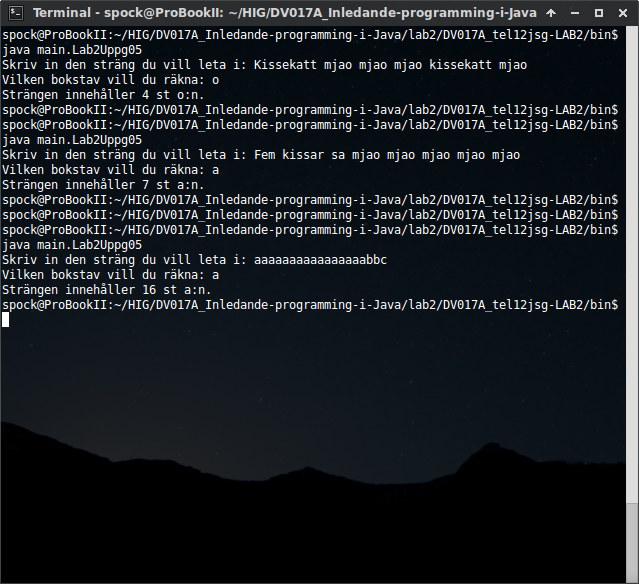
\includegraphics[width=\linewidth]{img/05.png}
    \caption{Körning av koden till Uppgift~\ref{sec:uppg05}}
    \label{fig:uppg05-screenshot}
\end{figure}
% TODO: Lägg till skärmdump av #05.

